\newpage
\section{实验结果及分析}
\subsection{ALU验证实验结果}
8位num1输入后无符号拓展为32位
\begin{table}[htbp]
    \centering
    \caption{ALU结果表}
    \begin{tabular}{c|c|c}
        \hline
        操作            &	Num1        &	Result\\
        \hline
        A + B(Unsigned) &	8’b00000010 & 	32'h00000003\\
        A - B           &	8’b11111111 &	32'h000000FE\\
        A AND B         &	8’b11111110 &	32'h00000000\\
        A OR B          &	8’b10101010 &	32'h000000AB\\
        $\overline{A}$  &	8’b11110000 &	32'hFFFFFF0F\\
        SLT             &	8’b10000001 &	32'h00000000\\
        \hline
    \end{tabular}
    \label{tab:my1}
\end{table}

\subsection{流水线阻塞(暂停)仿真图}
\begin{figure}[htbp]
    \centering
    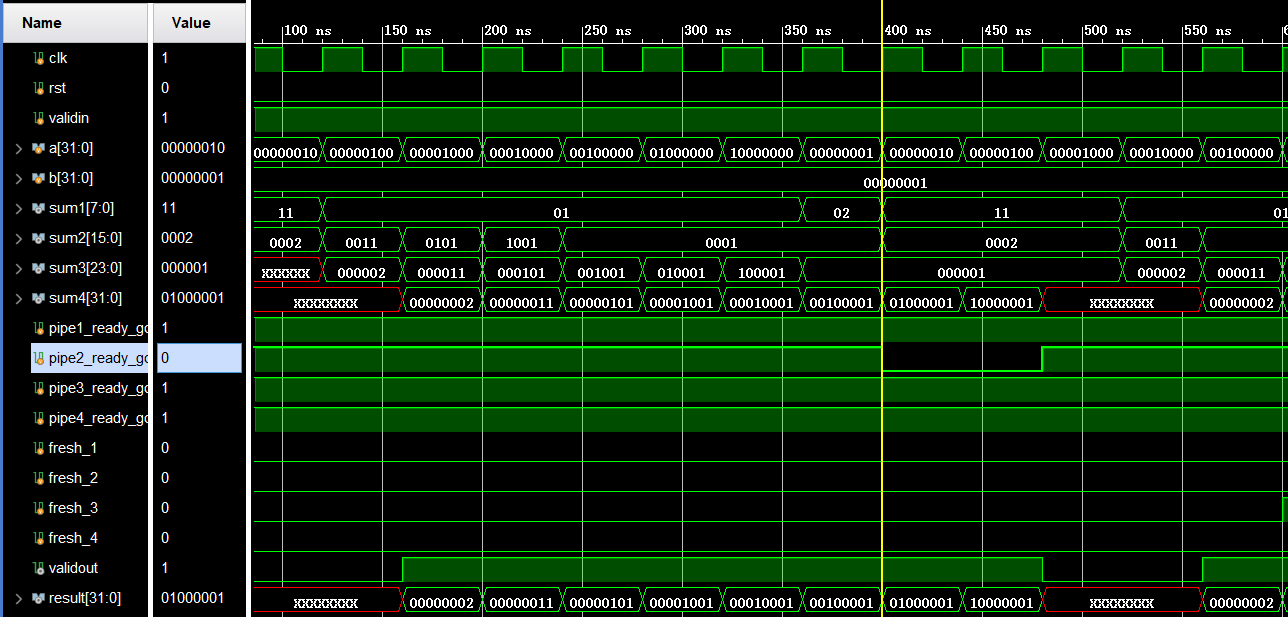
\includegraphics[width=0.9\textwidth]{stop.png}
    \caption{暂停}
    \label{fig:2}
\end{figure}

\subsection{结果分析}
通过该仿真图,我们发现每一个周期,流水线将计算各部分的值,在第四个周期得到最终的运算结果。而第二级暂停时,我们发现第一级流水线也将暂停,保留在一级流水线中的数据不变。第三级,第四级流水线继续运转直到无数据推进,此时,validout信号变为低电平。

\subsection{流水线刷新(清空)仿真图}
\begin{figure}[htbp]
    \centering
    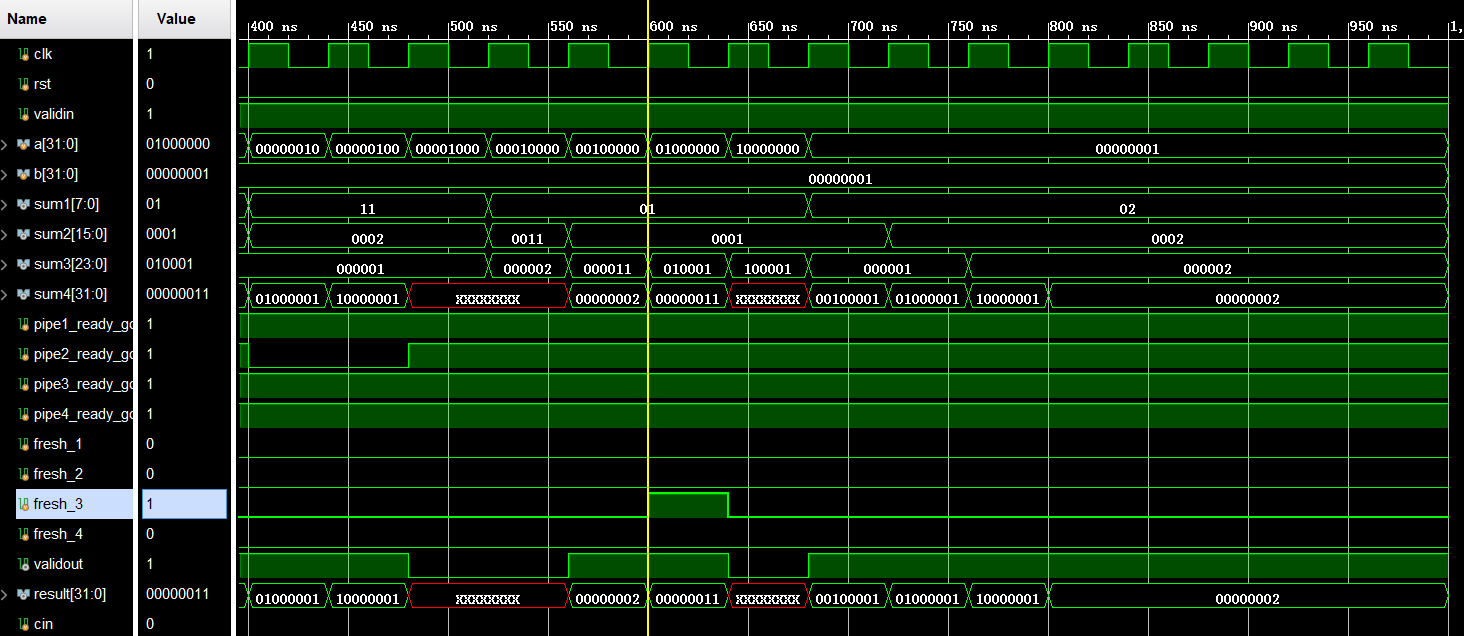
\includegraphics[width=0.9\textwidth]{fresh.png}
    \caption{刷新}
    \label{fig:3}
\end{figure}

\subsection{结果分析}
第三级刷新时,我们发现第一、二级流水线不受影响,但由于第三级流水线的刷新,导致下一周期第四级流水线无法得到数据,此时,validout信号为低电平。